\chapter{Gerenciar Solicitações da Unidade}
\label{detalhes:ger-os-unid}

\section{Introdução}

Conforme introdução, o módulo \textbf{``Gerenciar Solicitações da Unidade''} é uma tela muito parecida com o módulo já desenvolvido ``Gerenciar e Analisar Solicitações''. 

Seu objetivo é funcionar como uma ``caixa de entrada de solicitações'' para cada unidade interna da \ASSEL: UCJ, URP, UEF, USE e UDA.


	\begin{importante}{Cinco módulos em um}
		É importante ressaltar que será desenvolvido um único módulo que deverá atender as 5 unidades internas da \ASSEL. Assim, na perspectiva do usuário, é como se existissem 5 módulos ``Gerenciar Solicitações da Unidade'' separados - um para cada unidade interna. Na perspectiva do desenvolvedor, será desenvolvido um único módulo cujas informações apresentadas são filtradas através de um dropdown no canto superior direito da tela em que se escolherá em qual unidade (e portanto em qual módulo) o usuário está.
	\end{importante}


	De forma resumida, nesse módulo deverão ser mostradas todas as solicitações que estão naquela unidade selecionada no dropdown, o \textbf{estado na unidade}, os consultores atuando na qualidade de elaboradores, consultores atuando na qualidade de revisores além de informações internas como, por exemplo, prioridade interna e o tempo da solicitação na unidade desde o instante em que a solicitação foi entregue. Além dessas informações, o módulo deverão contar com botões para acessar funcionalidades de gerenciamento e controle das solicitações. Trata-se de uma tela de monitoração pois as solicitações serão exibidas na tabela enquanto estiverem sendo trabalhadas na unidade. Um mesmo consultor pode atuar como elaborador ou revisor em diferentes solicitações ao mesmo tempo. Contudo, ele nunca deverá acumular os dois papéis para uma mesma solicitação.

	Na seção a seguir detalhamos melhor os componentes do módulo.

\section{Conjuntos de componentes}

	\begin{center}
		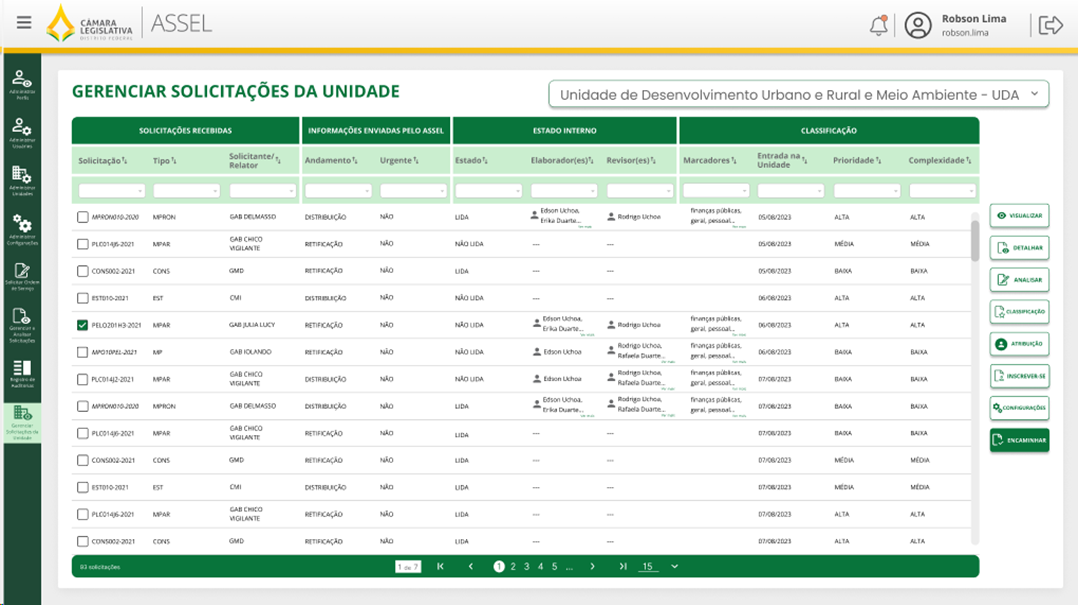
\includegraphics[width=0.9\textwidth]{fig/ger-sol-unid/GerenciarSolicitacoesUnidades27092023.png}
	\end{center}

	Conforme pode ser visto no protótipo, o módulo ``Gerenciar Solicitações da Unidade'' terá 3 conjuntos de componentes:
	
	\begin{itemize}
		\item \textbf{Dropdown de escolha da unidade}: Utilizado para escolher dentre as unidades internas, qual apresentar as informações de interesse;
		\item \textbf{Tabela de solicitações da unidade};
		\item \textbf{Botões para acesso de funcionalidades};
		\item \textbf{Modais para implementação de funcionalidades};
	\end{itemize}

	\subsection{Dropdown} 
	
	Conforme especificado, o dropdown superior direito permite alternar entre as unidades internas de modo que as informações exibidas na tabela de solicitações seja filtrada para exibir somente as informações das solicitações da unidade escolhida.
	
	\begin{nota}{Observação}
		Na prática, quando o sistema estiver funcionando, um usuário não poderá participar de duas unidades internas ao mesmo tempo e assim ele poderá ver apenas uma opção na listagem do dropdown correspondente à unidade interna em que ele está inscrito. No entanto, durante o desenvolvimento, para fins de testes, será necessário atribuir mais de uma unidade a um mesmo usuário e, portanto, este componente será usado para poder escolher qual módulo abstrato de qual unidade o usuário poderá acessar. 
	\end{nota}

	Dessa forma, os valores possíveis serão provenientes do módulo ``Gerenciar Unidades'' limitados às \textbf{unidades internas} atribuídas a determinado usuário.
	
	\begin{exemplo}{Exemplo}
		Suponha que determinado usuário esteja cadastrado nas unidades: Labhinova, ASSEL, UDA, USE e Gabinete do Deputado Delmasso. Dessas unidades, apenas as unidades UDA e USE são unidades internas. Dessa forma, quando o usuário acessar o módulo de gerenciamento de solicitações da unidade, ele só poderá ver as seguintes opções para escolha na lista do dropdown: UDA e USE.		
	\end{exemplo}

	\subsection{Tabela de Solicitações da Unidade} 	
	
	A tabela de solicitações pode ser vista no protótipo. 

	Ela basicamente lista as solicitações que foram enviadas para aquela unidade interna da \ASSEL \xspace e fornece colunas com informações da solicitação dividas em 3 grupos de colunas:


	
	\begin{itemize}
		\item \textbf{Solicitações Recebidas}: São colunas que exibem as propriedades da solicitação como o código identificador da solicitação, tipo e a unidade solicitante ou relator. 
		
		\item \textbf{Informações Enviadas pela ASSEL}: Como o remetente é sempre a ASSEL, as únicas colunas necessárias deste grupo são: \textbf{Andamento} e \textbf{Urgente}.
		
		\item \textbf{Estado Interno}: Trata-se de colunas com informações sobre o estado interno de elaboração do trabalho nesta unidade. Aqui planeja-se ter as seguintes colunas: 
		\begin{itemize}
			\item \textbf{Estado}: Exibe o estado interno propriamente dito em que uma solicitação encontra-se na unidade.
			\item \textbf{Elaborador(es)}: Uma solicitação poderá estar atribuída a múltiplos elaboradores e múltiplos revisores ao mesmo tempo. Assim, esta coluna deverá exibir os \CLs que estão atuando na solicitação na qualidade de \textbf{elaborador}. 
			\item \textbf{Revisore(es)}: Da mesma forma, esta coluna deverá exibir os \CLs que estão atuando na solicitação na qualidade de \textbf{revisor}. 
		\end{itemize}



		\item \textbf{Classificação}: São colunas para classificação e gerenciamento interno das solicitação na unidade:
			\begin{itemize}
				\item \textbf{Marcadores}: Permite que uma ou mais \emph{tags} ou marcadores de classificação sejam atribuídos a uma solicitação. O intuito é oferecer uma forma de classificar as solicitações com palavras chave. Os marcadores são conjuntos de termos atribuídos à solicitação de modo que solicitações com mesmos marcadores possam ser encontradas utilizando-se o filtro. 

				\item \textbf{Entrada na Unidade}: Exibe a a data em que a solicitação chegou na unidade.

				\item \textbf{Prioridade}: Classificação interna da prioridade da solicitação dentro da unidade em 3 níveis: Baixa, Média ou Alta.
				
				\item \textbf{Complexidade}: Classificação interna da complexidade da solicitação dentro da unidade em 3 níveis: Baixa, Média ou Alta.	
			\end{itemize}
	\end{itemize}

	\subsection{Botões} 	

	\begin{itemize}
		\item \textbf{Visualizar}: Tanto CLs quanto Supervisores podem acessar - Acessa modal de visualização do andamento - Se o estado é ``Não Lido'' e o Supervisor o acessa, gera a ação que tira do estado ``Não Lido'' para ``Em Análise''.
	
		\item \textbf{Detalhes}: Abre aba com detalhes das solicitaçõ(es) abertas. Já foi feito.

		\item \textbf{Analisar}: Botão de acesso exclusivo dos supervisores que permite acessar o modal de análise. Neste modal o supervisor decide se aceita a solicitação ou se devolve-a para a Assessoria Legislativa.
	
		\item \textbf{Atribuições}: Dá acesso a um modal de gerenciamento de atribuições com duas abas. 	Se o estado é ``Não Lido'' e o Supervisor o acessa, gera a ação que tira do estado ``Não Lido'' para ``Em Análise''.	
		
		\begin{itemize}
			\item \textbf{Gerenciar Atribuições}: Controle de Atribuições de Elaboradores e Revisores de uma dada solicitação selecionada. 

			\item \textbf{Gerenciar Inscrições}: Controle de Inscrições de Elaboradores e Revisores de uma dada solicitação selecionada. Esse botão só estará acessível caso alguma das configurações de dispensa de consentimento não esteja habilitada, ou seja, caso o supervisor precise consentir para aceitar uma  auto-atribuição. 
		\end{itemize}

	
		\item \textbf{Inscrever-se}: Modal para que tanto CLs quando Supervisores possam se inscrever em uma dada Solicitação na qualidade de elaborador ou revisor. Esse botão só pode ser utilizado se o estado for ``Na Fila'' ou ``Em Elaboração''. Esse botão só estará disponível caso isso esteja configurado nas opções da unidade. 
	
		\item \textbf{Classificação}: Botão de acesso exclusivo dos supervisores que permite acessar modal de escolha da prioridade, complexidade e gerenciamento de marcadores da solicitação selecionada.
	
		\item \textbf{Encaminhar}: Botão de acesso exclusivo dos supervisores que permite encaminhar para a ASSEL um ou mais solicitações que estão no estado final ``Solicitação Concluída''.		
	\end{itemize}
	
	\subsection{Modais}

	Alguns botões dão acesso a modais para implementar funcionalidades mais complexas: 
	
	\begin{itemize}
		\item \textbf{Modal Visualizar}: Modal idêntico ao que foi criado no Módulo ``Gerenciar e Analisar Solicitações'' para que seja visto as informações do andamento da solicitação selecionada. Um por vez. 
		
		\item \textbf{Aba Gerenciar Atribuições}: Modal de acesso exclusivo do chefe que permite gerenciar, para uma dada solicitação, quem sãos os elaboradores e revisores atuais. Mudanças realizadas usando esse modal devem ser registrados na árvore de histórico.
		
		\item \textbf{Aba Gerenciar Inscrições}: Modal de acesso exclusivo do chefe que permite visualizar para uma dada solicitação quem se inscreveu para atuar na solicitação como elaborador ou revisor e permite aceitar ou rejeitar essa inscrição.  Eventos realizados por meio deste modal devem ser registrados na árvore de histórico.		

		\item \textbf{Analisar}: Modal de acesso exclusivo do chefe que permitirá analisar uma solicitação e escolher uma ação que pode ser colocar a solicitação em um determinado estado ou mesmo realizar a operação de ``retorno'', ou seja, a devolução de solicitações para a ASSEL em casos em que a solicitação foi julgada como não pertencente à unidade. 
		
		\item \textbf{Gerenciar Configurações}: Modal de acesso exclusivo do supervisor que permitirá modificar as configurações da unidade.
	
	\end{itemize}


\section{Usuários que poderão acessar o módulo}

Os usuários que poderão acessar o módulo ``Gerenciar e Analisar Solicitações'' devem ser todos os usuários que estiverem inscritos numa mesma unidade interna e que possuírem os perfis de supervisor de unidade \hypertarget{data230823mudanca2}{\textbf{e/ou consultor da unidade}}. 

Na prática não haverá o perfil chefe e sim o perfil de supervisor. O chefe e o substituto devem atribuir para sí o perfil de supervisor de unidade. Isso permite em casos excepcionais que um chefe de unidade delegue para outra pessoa os poderes de supervisor e uma unidade interna poderia contar com mais de 2 supervisores ao mesmo tempo.

\section{Estados das solicitações}

Haverá um fluxo de estados internos que controla os estados de uma solicitação dentro da unidade conforme figura abaixo:

\begin{center}
	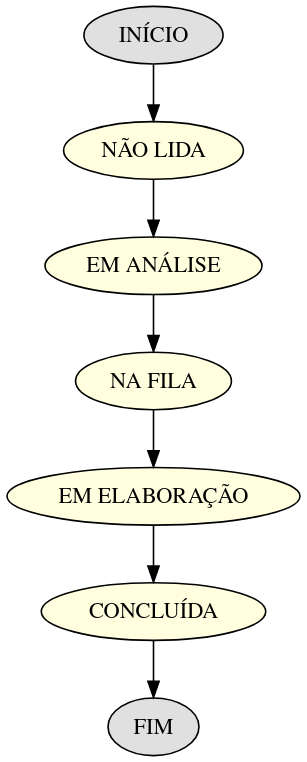
\includegraphics[width=0.2\textwidth]{fig/fluxoBasico.png}
\end{center}

\subsection{Estado ``Não Lida''}

\subsubsection*{Descrição}

Situação que indica que a solicitação foi enviada pela ASSEL para a Unidade, a solicitação já está na tabela da unidade mas o Supervisor da Unidade ainda não tomou ciência.

\subsubsection*{Como entra?}

\begin{itemize}
	\item Unidade ASSEL envia a solicitação para a Unidade com andamento específico. 
	\item Solicitação desaparece da caixa de entrada da Assel e aparece na caixa de entrada da Unidade.
\end{itemize}

\subsubsection*{Como sai?}

Supervisor da Unidade seleciona a Solicitação e clica em ``Visualizar'' ou em ``Gerenciar Atribuições'' ou ainda em ``Analisar''.

\subsection{Estado ``Em Análise''}

Trata-se do estado seguinte ao estado ``Não Lido'' indicando que o Supervisor da Unidade leu e tomou ciência da solicitação que chegou na unidade. Aqui o supervisor deverá tomar algumas atitudes:

\begin{itemize}
	\item Manter nesse estado sinalizando que a decisão ainda não foi tomada;
	\item Acessar modal de análise e mudar para estado ``Na Fila'' permitindo que a atribuição de elaboradores e revisores se inicie;
	\item Acessar Modal de Gerenciamento de Atribuições para ela mesma escolher os elaboradores que deverão trabalhar nessa solicitação;
	\item Acessar modal de análise para providenciar um retorno caso julgue que a solicitação não pertence ou não pode ser atendida na unidade.
\end{itemize}

Aqui teremos que fazer um modal de Análise parecido com aquele utilizado pela Assel para ajudar o Supervisor da Unidade a tomar essa decisão. Aqui ocorre a possibilidade do retorno que é quando o Supervisor devolve a solicitação para Assel por diversos motivos.


\subsection{Estado: ``Na Fila''}

Solicitações no estado ``Na Fila'' estão liberados para que \CLs se inscrevam na solicitação para serem elaboradores.

A atribuição ocorre de duas formas a depender da configuração da Unidade: Empurrar e Puxar.

\begin{itemize}
	\item \textbf{Empurrar}: Chefe diz quem será o elaborador/revisor e em seguida, dependendo das configurações da unidade, o usuário atribuído precisa consentir ou rejeitar. 
	
	\item \textbf{Puxar}: O usuário se inscreve na solicitação e caso assim esteja configurado, ele	passa a ser o elaborador/revisor automaticamente ou segue para consentimento do chefe.
\end{itemize}


\begin{importante}{Acordo necessário antes de mudar o estado}
	Importante destacar que tanto no estilo ``empurrar'' quanto ``puxar'' de atribuição de elaboradores e revisores, deve haver acordo dentre o supervisor que atribuiu e o \CL que foi atribuído para que o estado seguinte seja atingido. A obrigatoriedade do consentimento do chefe na modalidade ``puxar'' será configurável para cada unidade. Por outro lado, quando o supervisor ``empurra'' uma atribuição, o \CL atribuído sempre terá a opção de aceitar ou rejeitar essa ação. Serão nessas interações entre supervisores e consultores que deveremos utilizar o sistema de notificações para que as todas as partes sejam notificadas das ações realizadas por cada um.
\end{importante}


\subsection{Estado: ``Em Elaboração''}

O estado ``Em Elaboração'' é o estado que informa que uma dada solicitação está sendo elaborada por algum \CL. 

As seguintes regras deverão ser obedecidas:

\begin{enumerate}
	\item Solicitações que já estão no estado ``Em Elaboração''  pode ocorrer a entrada e saída de outros elaboradores.

	\item Solicitações que já estão no estado ``Em Elaboração''  pode ocorrer a entrada e saída de outros revisores.
	
	\item Caso uma solicitação esteja no estado ``Em Elaboração'' com apenas um \hypertarget{data230823mudanca1}{\textbf{único elaborador e ele desejar desistir}}, então os supervisores da unidade serão notificados dessa desistência. \textbf{E, além disso, quaisquer revisores que, por ventura estiverem atribuídos à solicitação, eles serão desatribuídos com envio de notificação informando-os sobre essa desatribuição.} E o estado da solicitação voltará a ser ``Na Fila''.
	
	\item No momento da atribuição na modalidade ``empurrar'', deverá ser informado obrigatoriamente em qual qualidade o \CL está sendo atribuído: elaborador ou revisor. 
	
	\item Na modalidade ``puxar'', a primeira pessoa que se inscreve na solicitação deve ser na qualidade de elaborador.
	
	\item Portanto, seja qual for a modalidade de atribuição, o sistema não vai permitir que um revisor seja atribuído a uma solicitação que ainda não possua, no mínimo um elaborador.
	
	\item Todo \CL pode atuar como elaborador ou revisor de diferentes solicitações ao mesmo tempo;
	
	\item Contudo, um \CL não pode atuar ao mesmo tempo como elaborador e revisor de uma mesma solicitação.
	
	\item Um \CL que participou da elaboração de uma solicitação na qualidade de elaborador e saiu não poderá voltar como revisor, apenas como elaborador.
	
	\item Um \CL que participou da elaboração de uma solicitação na qualidade de revisor e saiu não poderá voltar como elaborador, apenas como revisor.
	
	\item Somente elaboradores podem fazer upload dos documentos finais.
	
	\item O comportamento padrão será de não permitir que seja feito o upload dos documentos finais caso não haja, atribuído à solicitação, no mínimo um \CL na qualidade de revisor.	
	
	\item No modal de análise, para cada solicitação, haverá a opção de \hypertarget{data250823mudanca1}{remover a obrigação de haver pelo menos um revisor de modo a liberar o upload dos documentos finais}. Assim, o supervisor pode configurar essa opção separadamente para cada solicitante permitindo em casos de urgência ou na falta de \CLs que uma solicitação seja concluída mesmo sem ter sido atribuído a ela um \CL na qualidade de revisor.
	
	
	
\end{enumerate}

\subsubsection{A Revisão ocorre dentro da Elaboração}

\hypertarget{data230823mudanca3}{Inicialmente pensou-se em criar um estado separado} \emph{``Em Revisão''} que ocorreria ao final do estado ``Em Elaboração''. 

Contudo, a diversidade de estilos de formas e metodologias utilizadas para desenvolver os trabalhos de elaboração e revisão em cada uma das 5 unidades mostrou que tentar sistematizar o trabalho tentando-se criar estados separados de elaboração e revisão iria acabar limitando e restringindo as diversas dinâmicas de trabalho atualmente em vigor nas unidades internas da Assessoria Legislativa.

Por exemplo, algumas unidades fazem uma revisão apenas ao final da elaboração do documento. Contudo, outras unidades preferem fazer uma ou mais rodadas separadas de revisão por revisores diferentes. Algumas unidades preferem constituir a equipe de elaboração e revisão de uma única vez enquanto em outras unidades os revisores são escolhidos apenas quando os elaboradores sinalizam que finalizaram os trabalhos. E finalmente, independente da metodologia de elaboração e revisão escolhida, o documento revisado precisa voltar para as mãos dos elaboradores que deverão decidir por acatar ou rejeitar as propostas de melhorias dos colegas.
 
Dessa forma, para que o sistema seja flexível e não limite a liberdade de escolha das dinâmicas de trabalho das unidades, decidiu-se tratar a revisão como um trabalho que ocorre dentro do estado ``Em Elaboração'' de modo que, quando a elaboração termina, significa que a revisão também já aconteceu e os artefatos de entrega encontram-se na versão final para serem entregues para o solicitante.

% Manter a flexibilização das dinâmicas de elaboração e revisão dos trabalhos




\subsection{Estado: ``Conclusão da Solicitação''}

É o caso quando a solicitação que encontra-se no estado interno ``Em Elaboração'' e algum dos elaboradores escolhe fazer o upload dos arquivos finais e esse upload é permitido e realizado. 

Solicitações no estado ``Conclusão da Solicitação'' são elegíveis para serem encaminhados de volta para a ASSEL com o andamento de mesmo nome ``Conclusão da Solicitação''. 

Contudo, esse encaminhamento só pode ser feito pelos usuários com perfil de supervisores da unidade. O encaminhamento é feito selecionando uma ou mais solicitações com estado  ``Conclusão da Solicitação'' e clicando-se no botão ``Encaminhar'' que por sua vez abrirá modal de encaminhamento semelhante àquele desenvolvido no módulo ``Gerenciar e Analisar Solicitações''.

\section{Configurações}


\begin{nota}{Atenção: Seção Desatualizada}
	Essa seção está desatualizada! Essa funcionalidade já evoluiu para melhorar o formato de escolha dentre as diferentes configurações. Essa seção foi deixada aqui para que seja possível entender como as configurações  deverão funcionar. 
	
	\tcblower
	
	Utilizar como referência os slides da apresentação e os protótipos atualizados para verificar as opções de configuração existentes.
\end{nota}

Para permitir que diferentes unidades escolham seus estilos de gerenciamentos de atividades, alguns comportamentos dos módulos serão habilitados e desabilitados por variáveis de configuração.

Assim, toda unidade terá as seguintes configurações:

\subsection{Permitir inscrição de CLs na qualidade de elaborador nas solicitações}

\begin{itemize}
	\item Permite que os CLs daquela unidade se inscrevam como elaboradores nas solicitações com estado ``Na Fila''. Isto é a auto-atribuição como elaborador;
	
	\item Valor booleano: Sim ou Não.	
\end{itemize}

\subsubsection{Dispensar consentimento do supervisor quando ocorrer a inscrição na qualidade de elaborador}

Esta será uma opção que só faz sentido se ``Permitir inscrição de CLs na qualidade de Elaboradores nas solicitações'' for verdadeiro.

\begin{itemize}
	\item Valor booleano: Sim ou Não.	
\end{itemize}

Ou seja, o comportamento padrão é que se uma unidade permite que os CLs dessa unidade se inscrevam numa solicitação na qualidade de elaborador, o estado seguinte depende do consentimento do supervisor. Mas se a configuração ``Dispensar consentimento'' estiver habilitada, então essa etapa do consentimento não ocorre, ou seja, o consentimento é automático.

\subsection{Permitir inscrição de CLs na qualidade de revisor nas solicitações}

\begin{itemize}
	\item Permite que os CLs daquela unidade se inscrevam como revisores nas solicitações com estado ``Em Elaboração''. Isto é a auto-atribuição como revisor;
	
	\item Valor booleano: Sim ou Não.	
\end{itemize}

\subsubsection{Dispensar consentimento do supervisor quando ocorrer a inscrição na qualidade de revisor}

Idem.

\subsection{Resumo das variáveis de configuração de uma unidade}

Então serão 4 variáveis para cada unidade. Como temos 5 unidades, o sistema deve manter o estado de $4x5 = 20$ variáveis ao todo. As variáveis são:

\begin{itemize}
	\item \msnao \textbf{Permitir} inscrição de consultores na qualidade de \textbf{elaborador} das solicitações;
	\item \msnao \textbf{Dispensar consentimento} de supervisor para inscrição de consultores na qualidade de \textbf{elaborador} das solicitações;
	\item \msnao \textbf{Permitir} inscrição de consultores na qualidade de \textbf{revisor} das solicitações;
	\item \msnao \textbf{Dispensar consentimento} de supervisor para inscrição de consultores na qualidade de \textbf{revisor} das solicitações;
\end{itemize}





\section{Modalidades de Atribuição}

Como já foi apresentado ao longo das seções anteriores, no que tange a funcionalidade de atribuição, iremos desenvolver os dois modos: ``puxar'' e ``empurrar''.

\subsection{Empurrar}

A modalidade de atribuição ``empurrar'' consiste em um supervisor que deseja atribuir uma solicitação para um ou mais \CLs elaborarem e um ou mais \CLs revisarem.

Essa funcionalidade sempre estará disponível para o supervisor e essa ação sempre deve passar pelo aceite ou rejeição do \CL. 

\subsection{Puxar}

A modalidade de atribuição ``puxar'' consiste em um \CL que ao acessar o módulo vê uma lista de solicitações no estado ``Na Fila'' ou ``Em Elaboração''. 

O estado ``Na Fila'' indica que a solicitação já foi liberada pelo supervisor para elaboração, mas até o momento ninguém iniciou sua elaboração. 

O estado ``Em Elaboração'' indica que a solicitação já está sendo elaborado por alguém e até mesmo já há possivelmente revisores trabalhando nela. 

Seja qual for o estado, a modalidade ``puxar'' permite que um \CL se inscreva numa solicitação nesses estados indicando a qualidade que deseja atuar de elaborador ou revisor.  

A modalidade de atribuição ``puxar'' será habilitada pela variável de configuração. Se habilitado, então o consentimento do supervisor deve ocorrer por padrão a não ser que a configuração de dispensa de consentimento também esteja configurada para verdadeiro.

\section{Modalidades de Desatribuição}

\hypertarget{data230823mudanca4}{Desistência e Desatribuição são funcionalidades} para que um \CL já alocado para uma solicitação em alguma qualidade seja desalocado. 

A diferença entre elas é de quem é a iniciativa:

\begin{itemize}
	\item A \textbf{desistência} é quando o \CL é desatribuído de uma solicitação por iniciativa dele.
	
	\item A \textbf{desatribuição} é quando um \CL é desatribuído de uma solicitação por iniciativa de um supervisor.
\end{itemize}

\subsection{Funcionalidades para desatribuir}

\subsubsection{Desistência}

A idéia é que a desistência seja automática. Ou seja, se um \CL quer desistir, ele não precisa do consentimento do supervisor. Ele clica em desistir, motiva e o sistema vai desatribuí-lo da solicitação automaticamente. Os supervisores serão notificados disso, contudo o efeito da desistência é imediato sem necessidade de aceitação ou reprovação de um supervisor.

\subsubsection{Desatribuição}

Na desatribuição um supervisor deseja remover um \CL do papel de elaborador ou revisor de uma dada solicitação. A idéia é de que nesse caso a desatribuição iniciada por um supervisor só seja efetivada após o consentimento (aprovação ou reprovação) do \CL desatribuído.

\subsubsection{Desatribuição Forçada}

É caso semelhante ao da desatribuição, contudo, o \CL não terá escolha e será removido da solicitação de forma imediata. Ele será notificado disso.

Esse caso seria usado pelo supervisor em casos em que o \CL desatribuído não tem condições de aceitar a desatribuição como por exemplo caso ele esteja afastado do trabalho e não há como acessar o sistema para aceitar ou reprovar a desatribuição. Ex.: Ficou doente e não pode acessar o sistema para aceitar a desatribuição.

\subsection{Como funcionaria}

No caso da desistência, já há um botão chamado ``desistir'' que, após uma dupla confirmação, abre um modal para o \CL informar o motivo da desistência.

No caso da desatribuição, quando o supervisor acessar o modal de atribuição, selecionar um \CL já alocado e clicar em ``remover'', abre-se um modal para ele escolher o motivo dentre opções pré-determinadas.

Se a opção escolhida para a motivação for ``Afastamento'' então o sistema faz a desatribuição forçada.

Se a opção escolhida for ``Outros'' com caixa de texto para o supervisor dizer porque está desatribuindo-o daquela solicitação, então o sistema faria a desatribuição normal, isto é, notificaria o consultor e aguardaria ele avaliar se aceita ou rejeita essa desatribuição.











 













